
%%%%%%%%%%%%%%%%%%%%%%%%%%%%%%%%%%%%%%%%%%%%%%%%%%%%%%%%%%%%%%%%%%%%
%%%%%%%%%%%%%JIBLM Formatting Package%%%%%%%%%%%%%%%%%%%%%%%%%%%%%%
%%%%%%%%%%%%%Version 1.2: August, 2008%%%%%%%%%%%%%%%%%%%%%%%%%%%
%%%%%%%%%%%%%Author: Paul J. Kapitza, Berry College%%%%%%%%%%%%%%%%
%%%%%%%%%%%%%%%%%%%%%%%%%%%%%%%%%%%%%%%%%%%%%%%%%%%%%%%%%%%%%%%%%%%

\documentclass[oneside]{book}
%%%%%%%%%%%%%journal additions%%%%%%%%%%%%%%%%%%%%%%%%%%%%%%%%%%%%%
\usepackage{time}%make system time available
\usepackage{enumerate}%extended enumeration package
%%%%%%%%%%%%%Symbol libraries%%%%%%%%%%%%%%%%%%%%%%%%%%%%%%%%%%%%%
\usepackage{amssymb}
\usepackage{amsmath}
\usepackage{latexsym}
\usepackage{amsthm}%extended ams-theorem environment

\usepackage{lettrine}%Drop-caps for Masthead
\usepackage{mathptmx}%Times Roman type package for both math and text


\usepackage{endnotes}%Footnotes to the instructor.
   
   
   
   
%%%%%%%%%%%%%Header Customization%%%%%%%%%%%%%%%%%%%%%%%%%%%%%%%%%
\usepackage{fancyhdr}%Header customization
\pagestyle{fancy}
%%%%%%%%%%%%%Chapter headings%%%%%%%%%%%%%%%%%%%%%%%%%%%%%%%%%
\renewcommand{\chaptermark}[1] {\markboth{#1}{}}%

%%%%%%%%%%%%%Page Formatting%%%%%%%%%%%%%%%%%%%%%%%%%%%%%%%%%%
\setlength{\oddsidemargin}{63pt}%%%%%One-sided printing values for 10pt. text-Remove for two sided print
\setlength{\evensidemargin}{63pt}%%%%%One-sided printing values for 10pt. text-Remove for two sided print

\setlength{\parskip}{1mm}
\setlength{\textwidth}{5.0in}
\setlength{\textheight}{8.0in}

%%%%%%%%%%%%%%%%%%%%%%%%%%%%AUTHOR MASTHEAD%%%%%%%%%%%%%%%%%%%%%%%%%%%%%
\newcommand{\authormasthead}{
\begin{flushleft}
\hspace{8.0mm}
\rule{0.3\linewidth}{0.3mm}
\lettrine[lines=2]{D}{raft \rule[3pt]{10mm}{0.5pt} Draft \rule[3pt]{10mm}{0.5pt} Draft \rule[3pt]{10mm}{0.5pt} Draft}
\rule{0.3\linewidth}{0.3mm}
%\hspace{1mm} Issue~\textbf{#1}, Volume #2        Issue 1 (August, 2007)
\vspace{0.2in}
\end{flushleft}
}
%%%%%%%%%%%%%%%%%%%%%%%%%%%%AUTHOR MASTHEAD%%%%%%%%%%%%%%%%%%%%%%%%%%%%%

%%%%%%%%%%%%%%%%%%%%%%%%%%%%TIMESTAMP%%%%%%%%%%%%%%%%%%%%%%%%%%%%%
%%Uses the ``time" package to stamp the time-Editing Feature
\newcommand{\timestamp}{{Edited: \texttt{\now , \today}}}
%%%%%%%%%%%%%%%%%%%%%%%%%%%%TIMESTAMP%%%%%%%%%%%%%%%%%%%%%%%%%%%%%


\let\affiliation\date


%%%%%%%%%%%%%%%%%%%%%%%%%%%% TITLEPAGE%%%%%%%%%%%%%%%%%%%%%%%%%%%%%
%
\makeatletter
\def\maketitle{%
  \null
  \thispagestyle{empty}%
  \timestamp
  \authormasthead
  %\vfill
  \normalfont
  \vspace{2in}
\begin{center}\leavevmode
{\Huge \@title\par}%
\vspace{20mm}
{\Large \@author\par}%
\vspace{5mm}
{\Large \@date\par}% pass affiliation
{\Large \ }
\end{center}
  \vfill
  \null
  \cleardoublepage
 \let\newauthor\@author%transfer to footer line
 }%
\makeatother
%%%%%%%%%%%%%%%%%%%%%%%%%%%% END OF TITLEPAGE%%%%%%%%%%%%%%%%%%%%%%%%%%%%%

%Customized headers and footers- replace authorname with register
\lhead{ \leftmark} \chead{} \rhead{\thepage}
\lfoot{\newauthor} \cfoot{} \rfoot{\emph{DRAFT -- DRAFT -- DRAFT}}
\renewcommand{\headrulewidth}{0.4pt}
\renewcommand{\footrulewidth}{0.4pt}
%
%%%%%%%%%%%%%%%%%%%%%%%%%%%% Annotation Environment %%%%%%%%%%%%%%%%%%%%%%%%%%%%%
\usepackage{comment}
\newcommand{\InstructorVersion}{\includecomment{annotation}}
\newcommand{\StudentVersion}{\excludecomment{annotation}}
%%%%%%%%%%%%%%%%%%%%%%%%%%%% END OF Annotation Environment%%%%%%%%%%%%%%%%%%%%%%%%%%%%%



%%%%%%%%%%%%%%%%%%%%%%%%%%%% Begin--Sectioning Redefines%%%%%%%%%%%%%%%%%%%%%%%%%%%%%
%
\makeatletter
\renewcommand{\@makechapterhead}[1]{%
\vspace*{50\p@}%
  {\parindent \z@ \raggedright \normalfont
    \ifnum \c@secnumdepth >\m@ne
      \if@mainmatter
        \huge \@chapapp\space \thechapter                
        \par\nobreak
        \vskip 20\p@
      \fi
    \fi
    \interlinepenalty\@M
    \LARGE\bfseries  #1\par\nobreak                        
    \vskip 40\p@
  }}


\renewcommand{\@makeschapterhead}[1]{%
  \vspace*{50\p@}%
  {\parindent \z@ \raggedright
    \normalfont
    \interlinepenalty\@M
    \LARGE\bfseries  #1\par\nobreak                      
    \vskip 40\p@
  }}

\makeatother
%%%%%%%%%%%%%%%%%%%%%%%%%%%% End--Sectioning Redefines%%%%%%%%%%%%%%%%%%%%%%%%%%%%%




%%%%%%%%%%Theorem Environments%%%%%%%%%%%%%%%%%%%%%%%%
\newtheorem{theorem}{Theorem}
\newtheorem{acknowledgment}[theorem]{Acknowledgment}
\newtheorem{algorithm}[theorem]{Algorithm}
\newtheorem{axiom}[theorem]{Axiom}
\newtheorem{case}[theorem]{Case}
\newtheorem{claim}[theorem]{Claim}
\newtheorem{conclusion}[theorem]{Conclusion}
\newtheorem{condition}[theorem]{Condition}
\newtheorem{conjecture}[theorem]{Conjecture}
\newtheorem{corollary}[theorem]{Corollary}
\newtheorem{criterion}[theorem]{Criterion}
\newtheorem{definition}[theorem]{Definition}
\newtheorem{example}[theorem]{Example}
\newtheorem{exercise}[theorem]{Exercise}
\newtheorem{lemma}[theorem]{Lemma}
\newtheorem{notation}[theorem]{Notation}
\newtheorem{problem}[theorem]{Problem}
\newtheorem{proposition}[theorem]{Proposition}
\newtheorem{remark}[theorem]{Remark}
\newtheorem{solution}[theorem]{Solution}
\newtheorem{summary}[theorem]{Summary}
%%%%%%%%%%Theorem Environments%%%%%%%%%%%%%%%%%%%%%%%%
%%%%%%%%%%%%%%%%%%%%%%%%%%%%%%%%%%%%%%%%%%%%%%%%%%%%%%%%%%%%%%%%%%%
%%%%%%%%%%%%%JIBLM Formatting Package%%%%%%%%%%%%%%%%%%%%%%%%%%%%%%
%%%%%%%%%%%%%Version 1.2: August, 2008%%%%%%%%%%%%%%%%%%%%%%%%%%%
%%%%%%%%%%%%%Author: Paul J. Kapitza, Berry College%%%%%%%%%%%%%%%%
%%%%%%%%%%%%%%%%%%%%%%%%%%%%%%%%%%%%%%%%%%%%%%%%%%%%%%%%%%%%%%%%%%%
% Modifications marked with DJH

\RequirePackage{xcolor} %% DJH (Otherwise you get a bunch of warnings)
\documentclass[oneside]{book}
%%%%%%%%%%%%%journal additions%%%%%%%%%%%%%%%%%%%%%%%%%%%%%%%%%%%%%
\usepackage{time}%make system time available
\usepackage{enumerate}%extended enumeration package
%%%%%%%%%%%%%Symbol libraries%%%%%%%%%%%%%%%%%%%%%%%%%%%%%%%%%%%%%
% DJH % \usepackage{amssymb}
\usepackage{amsmath}
\usepackage{latexsym}
\usepackage{amsthm}%extended ams-theorem environment

\usepackage{lettrine}%Drop-caps for Masthead
\usepackage{mathptmx}%Times Roman type package for both math and text


\usepackage{endnotes}%Footnotes to the instructor.

\usepackage[letterpaper, margin=1.0in]{geometry} % DJH: Wider margins
\usepackage[charter]{mathdesign} % DJH: Different font


%%%%%%%%%%%%%Header Customization%%%%%%%%%%%%%%%%%%%%%%%%%%%%%%%%%
\usepackage{fancyhdr}%Header customization
\pagestyle{fancy}
%%%%%%%%%%%%%Chapter headings%%%%%%%%%%%%%%%%%%%%%%%%%%%%%%%%%
\renewcommand{\chaptermark}[1] {\markboth{#1}{}}%

%%%%%%%%%%%%%Page Formatting%%%%%%%%%%%%%%%%%%%%%%%%%%%%%%%%%%
%DJH %\setlength{\oddsidemargin}{63pt}%%%%%One-sided printing values for 10pt. text-Remove for two sided print
%DJH %\setlength{\evensidemargin}{63pt}%%%%%One-sided printing values for 10pt. text-Remove for two sided print

\setlength{\parskip}{1mm}
% DJH % \setlength{\textwidth}{5.0in}
% DJH % \setlength{\textheight}{8.0in}

%%%%%%%%%%%%%%%%%%%%%%%%%%%%AUTHOR MASTHEAD%%%%%%%%%%%%%%%%%%%%%%%%%%%%%
\newcommand{\authormasthead}{
\begin{flushleft}
\hspace{8.0mm}
\rule{0.3\linewidth}{0.3mm}
\lettrine[lines=2]{D}{raft \rule[3pt]{10mm}{0.5pt} Draft \rule[3pt]{10mm}{0.5pt} Draft \rule[3pt]{10mm}{0.5pt} Draft}
\rule{0.3\linewidth}{0.3mm}
%\hspace{1mm} Issue~\textbf{#1}, Volume #2        Issue 1 (August, 2007)
\vspace{0.2in}
\end{flushleft}
}
%%%%%%%%%%%%%%%%%%%%%%%%%%%%AUTHOR MASTHEAD%%%%%%%%%%%%%%%%%%%%%%%%%%%%%

%%%%%%%%%%%%%%%%%%%%%%%%%%%%TIMESTAMP%%%%%%%%%%%%%%%%%%%%%%%%%%%%%
%%Uses the ``time" package to stamp the time-Editing Feature
\newcommand{\timestamp}{{Edited: \texttt{\now , \today}}}
%%%%%%%%%%%%%%%%%%%%%%%%%%%%TIMESTAMP%%%%%%%%%%%%%%%%%%%%%%%%%%%%%


\let\affiliation\date


%%%%%%%%%%%%%%%%%%%%%%%%%%%% TITLEPAGE%%%%%%%%%%%%%%%%%%%%%%%%%%%%%
%
\makeatletter
\def\maketitle{%
  \null
  \thispagestyle{empty}%
  \timestamp
  \authormasthead
  %\vfill
  \normalfont
  \vspace{2in}
\begin{center}\leavevmode
{\Huge \@title\par}%
\vspace{20mm}
{\Large \@author\par}%
\vspace{5mm}
{\Large \@date\par}% pass affiliation
{\Large \ }
\end{center}
  \vfill
  \null
  \cleardoublepage
 \let\newauthor\@author%transfer to footer line
 }%
\makeatother
%%%%%%%%%%%%%%%%%%%%%%%%%%%% END OF TITLEPAGE%%%%%%%%%%%%%%%%%%%%%%%%%%%%%

%Customized headers and footers- replace authorname with register
\lhead{ \leftmark} \chead{} \rhead{\thepage}
\lfoot{Hunter $<$ Morrow} \cfoot{} \rfoot{\emph{DRAFT -- DRAFT -- DRAFT}} %DJH
\renewcommand{\headrulewidth}{0.4pt}
\renewcommand{\footrulewidth}{0.4pt}
%
%%%%%%%%%%%%%%%%%%%%%%%%%%%% Annotation Environment %%%%%%%%%%%%%%%%%%%%%%%%%%%%%
\usepackage{comment}
\newcommand{\InstructorVersion}{\includecomment{annotation}}
\newcommand{\StudentVersion}{\excludecomment{annotation}}
%%%%%%%%%%%%%%%%%%%%%%%%%%%% END OF Annotation Environment%%%%%%%%%%%%%%%%%%%%%%%%%%%%%



%%%%%%%%%%%%%%%%%%%%%%%%%%%% Begin--Sectioning Redefines%%%%%%%%%%%%%%%%%%%%%%%%%%%%%
%
\makeatletter
\renewcommand{\@makechapterhead}[1]{%
\vspace*{50\p@}%
  {\parindent \z@ \raggedright \normalfont
    \ifnum \c@secnumdepth >\m@ne
      \if@mainmatter
        \huge \@chapapp\space \thechapter
        \par\nobreak
        \vskip 20\p@
      \fi
    \fi
    \interlinepenalty\@M
    \LARGE\bfseries  #1\par\nobreak
    \vskip 40\p@
  }}


\renewcommand{\@makeschapterhead}[1]{%
  \vspace*{50\p@}%
  {\parindent \z@ \raggedright
    \normalfont
    \interlinepenalty\@M
    \LARGE\bfseries  #1\par\nobreak
    \vskip 40\p@
  }}

\makeatother
%%%%%%%%%%%%%%%%%%%%%%%%%%%% End--Sectioning Redefines%%%%%%%%%%%%%%%%%%%%%%%%%%%%%




%%%%%%%%%%%Theorem Environments%%%%%%%%%%%%%%%%%%%%%%%%
%% \newtheorem{theorem}{Theorem}[chapter] % DJH
%\theoremstyle{definition} % DJH
%\newtheorem{acknowledgment}[theorem]{Acknowledgment}
%\newtheorem{algorithm}[theorem]{Algorithm}
%\newtheorem{axiom}[theorem]{Axiom}
%\newtheorem{case}[theorem]{Case}
%\newtheorem{claim}[theorem]{Claim}
%\newtheorem{conclusion}[theorem]{Conclusion}
%\newtheorem{condition}[theorem]{Condition}
%\newtheorem{conjecture}[theorem]{Conjecture}
%\newtheorem{corollary}[theorem]{Corollary}
%\newtheorem{criterion}[theorem]{Criterion}
%\newtheorem{definition}[theorem]{Definition}
%\newtheorem{example}[theorem]{Example}
%\newtheorem{exercise}[theorem]{Exercise}
%\newtheorem{lemma}[theorem]{Lemma}
%\newtheorem{notation}[theorem]{Notation}
%\newtheorem{proposition}[theorem]{Proposition}
%\newtheorem{remark}[theorem]{Remark}
%\newtheorem{solution}[theorem]{Solution}
%\newtheorem{summary}[theorem]{Summary}
%% \newtheorem{problem}{Problem} %DJH
%%%%%%%%%%Theorem Environments%%%%%%%%%%%%%%%%%%%%%%%%
 % My customized version
\usepackage{graphicx}
%
%%%%%%%%%%%%%%%%%%%%% Annotation Environment Switch%%%%%%%%%%%%
%\StudentVersion
\InstructorVersion
%%%%%%%%%%%%%%%%%%%%% Annotation Environment Switch%%%%%%%%%%%%
%

\begin{document}
\large
\frontmatter
\title{Abstract Algebra I \& II}
\author{David J. Hunter $<$ Margaret L. Morrow}
\affiliation{Westmont College}
\maketitle
\tableofcontents

%%%%%%%%%%%%%%%%%%%%%%%%%%%%%%%%%%%%To the Instructor%%%%%%%%%%%%%%%%%%%%%%%%%%%%%%%%

\begin{annotation}
 \chapter{To the Instructor}

These notes provide an introduction to abstract algebra for advanced undergraduate mathematics majors. There should be enough material for a two-semester sequence. At Westmont College, most mathematics majors and some minors take first semester of this sequence, which (ambitiously) covers Chapters 1--9. These chapters contain a fairly standard treatment of groups, rings, and fields. Some of the more motivated mathematics majors, including those destined for graduate school, will continue to the second semester, completing Chapters 10--13. The second semester includes some advanced group theory, including Sylow Theory, but its ultimate goal is to introduce students to Galois Theory.

This ultimate goal guides the selection of topics throughout these notes, beginning with the introductory activity. On the first day of class, students will discover how group operations can describe the symmetries of a polygon as permutations of the vertices. Analogously, by the end of the second semester, students will be using groups to describe automorphisms of splitting fields as permutations of the roots of a polynomial. It helps to keep the goal of the Galois correspondence in mind throughout both semesters, as it serves as a unifying theme.

At Westmont, enrollment for the first semester of this sequence is typically between 10 and 20, and second semester enrollment is much smaller. Regardless of class size, these notes are designed to be used with some form of the Moore method. Depending on the strength of the class, this method can be modified to provide additional support and scaffolding for students. I have found it very helpful to include the following components.
\begin{itemize}
    \item \textbf{Prework.} Before class, students should work independently on a selection of problems. I like to collect these preliminary solutions, either via online submissions or by running them through a scanner at the beginning of class. I grade these very leniently, giving full credit for what appears to be honest engagement with the problems. Currently, solutions to nearly every problem in every abstract algebra text can be found by searching the Internet, so lenient grading at this stage is essential. I tell students not to use any outside resources during the Prework stage, because I would rather see a half-right attempt at a problem of their own construction than a regurgitation of somebody else's solution.
    \item \textbf{Class Discussion.} During class, students will benefit by explaining their solutions, or lack thereof, to each other. These conversations can be encouraged in a variety of ways, using small-group discussion, class presentations, or a combination of the two. The goal of these discussions is to come to some consensus about a correct solution to each problem.
    \item \textbf{Postwork.} After class, students should be able to write up complete and correct solutions to every problem. These write-ups can be posted on a class wiki, maintained in a code repository, collected through a course management system, or kept in a journal. I carefully grade some subset of these assignments, where the subset size is determined by the size of the class.
\end{itemize}

Due to the abstract nature of the subject, it is important for instructors to provide some sort of regular framing and perspective on the material. Lectures will not be necessary, but students will appreciate hearing about why these techniques were developed and how these topics fit together.

The mathematical sophistication of the problems increases steadily throughout the sequence. Early on, students should be able to grapple with every detail of every proof. In later material, especially in the development of the Galois correspondence, some of the more difficult theoretical hurdles are given as theorems, with outlines, or ``sketches,'' of proofs. Often undergraduate treatments of Sylow and Galois theory simply state the main theorems and have students do calculations. While these notes do not require students to construct proofs of every theorem, they are designed to expose students to the theoretical development of the important results.

 Throughout the notes, you will notice superscripts at the end of some of the problems. These superscripts refer to endnotes in the last Chapter titled,
 ``Notes to the Instructor."

\section*{Acknowledgements}

Chapters 1--5 were originally written by Margaret Morrow and published on \texttt{jiblm.org}. These chapters have been modified, but retain much of her original content. The remainder of these notes were heavily influenced by some of my favorite algebra texts, including the following.
\begin{itemize}
    \item \textit{A First Course in Abstract Algebra}, by John Fraleigh.
    \item \textit{A First Course in Abstract Algebra}, by Joseph Rotman.
    \item \textit{Contemporary Abstract Algebra}, by Joseph Gallian.
    \item \textit{Algebra}, by Thomas Hungerford.
    \item \textit{Galois Theory}, by Joseph Rotman.
\end{itemize}

\end{annotation}


%%%%%%%%%%%%%%%%%%%%%%%%%%%%%%%%%%%%To the Student%%%%%%%%%%%%%%%%%%%%%%%%%%%%%%%%

\chapter{To the Student}

Have you ever wondered how modern mathematics came to be? To what extent are the definitions and theorems that we find in the canonical textbooks the result of choices made by historical figures? Is there something intrinsic to the subject that forces modern mathematical theory down the path that it takes? Put another way, would Earthling mathematicians recognize the work of a community of mathematicians from a distant galaxy?

We can glean some insight into these questions by proceeding axiomatically: make as few assumptions and definitions as possible, and see where logical deduction leads. The material in these notes represents the consequences of some very low-level mathematical foundations: logic, sets, and the integers. These consequences have applications throughout pure and applied mathematics, and are part of the \textit{lingua franca} of the discipline.

Historically, much of this subject was motivated by the search for solutions to polynomial equations: are there analogs to the quadratic formula for polynomials of degree greater than~2? It is easy to believe that our hypothetical space-alien mathematical colleagues would also be interested in this question. Throughout this semester and the next (should you persevere), you will be guided through a series of deductive discoveries along the path that modern mathematicians have blazed. Whether this path is the only reasonable one will be yours to judge once you have completed the journey.

\begin{quote}
  \textit{That student is taught the best who is told the least.} ---R. L. Moore
\end{quote}

These notes (along with the sequel) give a comprehensive coverage of two semesters of advanced undergraduate or beginning graduate algebra. However, these notes contain mostly questions, and you must supply the answers. Your written accounts of your inquiry and our class discussions will produce a complete abstract algebra textbook of your own construction.

\mainmatter

\chapter*{Introductory Activity}

\textbf{Example I: Symmetries.}
\begin{annotation}
 \endnote{The introductory activity is designed to be done in groups on the first day of class, after a brief explanation of symmetries. Later material will refer to the examples that it introduces, so it is important not to skip it. You may wish to prepare the cut-out triangles and squares in advance. (Tip: provide only one triangle and one square per group, to encourage collaboration.) This activity also gives students a chance to solve some relatively concrete problems in a relaxed atmosphere. Ideally, each group should be able to send a representative to the board to record their answers. In addition to presenting these useful examples, the goal is to get students accustomed to sharing their work with the rest of the class.}
\end{annotation}

We can think of a \textit{symmetry} of a plane figure as a rigid motion of the figure that results in the figure simply being repositioned on top of its original outline.

\textit{It is the final position of the figure that is important,} not the motion as such. For example, if we rotate the triangle below through $120^\circ$ or $480^\circ$, the triangle ends up in the same final position, so we do not think of these as distinct symmetries.

\begin{enumerate}
    \item Consider the symmetries of an equilateral triangle, as illustrated below. Each sketch shows the resulting position when the specified motion is applied to the triangle starting in the original position.
\begin{center}
    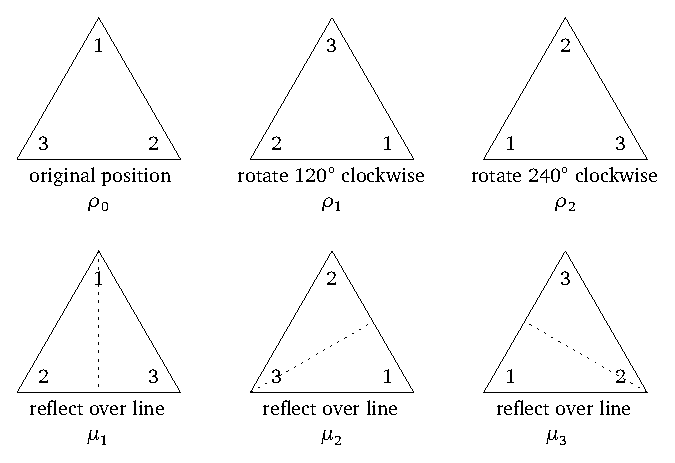
\includegraphics{wstriangles.eps}
\end{center}
    Cut an equilateral triangle out of a sheet of paper, and number the vertices 1, 2, and 3 as shown in the original position. Put the number of each vertex on the back of the triangle as well.

    We can apply one of the rigid motions, and then, \textit{continuing from the new position of the triangle,} apply another of the rigid motions. We can then record the overall effect as one of six symmetries listed above.

    For example if we first apply $\mu_1$, then (continuing from the resulting position) apply $\rho_1$ (a $120^\circ$ clockwise rotation) we end up with $\mu_2$. Using our usual function composition notation, we can write $\rho_1 \circ \mu_1 = \mu_2$.

    It is useful to write the results of all such combinations in table form, as shown below. We show the result of $\rho_1 \circ \mu_1$ in the row labeled $\rho_1$ and the column labeled $\mu_1$.

    \textbf{Important:} The convention is that we enter the result of $\rho_1 \circ \mu_1$ into the row corresponding to $\rho_1$ and the column corresponding to $\mu_1$, even though when we do these motions we first do the reflection $\mu_1$ and then the rotation $\rho_1$.

    \begin{center}
  \renewcommand{\arraystretch}{1.3}
    \begin{tabular}{|c||c|c|c|c|c|c|} \hline
        $\circ$ & $\rho_0$ & $\rho_1$ & $\rho_2$ & $\mu_1$ & $\mu_2$ & $\mu_3$ \\ \hline \hline
        $\rho_0$ & & & & & & \\ \hline
        $\rho_1$ & & & & & & \\ \hline
        $\rho_2$ & & & & & & \\ \hline
        $\mu_1$ & & & & & & \\ \hline
        $\mu_2$ & & & & & & \\ \hline
        $\mu_3$ & & & & & & \\ \hline
    \end{tabular}
    \end{center}

    Use the cut-out triangle to determine the result of all the compositions and complete the table. We will denote this collection of symmetries, together with composition, by $D_3$.

    \item You may have noticed that you can determine which symmetry was performed by looking at the labels of each vertex. Instead of representing rotations and reflections using Greek letters, it is often convenient to represent them using \textit{cycle notation.} For example, starting with the original position, the rotation $\rho_1$ moves vertex 1 to vertex 2, vertex 2 to vertex 3, and vertex 3 to vertex 1.
    \begin{center}
        
\includegraphics{d3cycles.eps}
    \end{center}
We can denote this rotation with the cycle $(1\; 2\; 3)$, which we read as ``1 goes to 2, 2 goes to 3, 3 goes to 1''. In cycle notation, each vertex moves to the one after it, and the last one wraps around to the first.

Complete the table below, giving the cycle that corresponds to each symmetry.
    \begin{center}
   \renewcommand{\arraystretch}{1.3}
    \begin{tabular}{|c|c|c|c|c|c|} \hline
         $\rho_0$ & $\rho_1$ & $\rho_2$ & $\mu_1$ & $\mu_2$ & $\mu_3$ \\ \hline
         $(1)$ & $(1\; 2\; 3)$ & $\phantom{(1\; 2\; 3)}$ & $(2\; 3)$ & $\phantom{(1\; 2\; 3)}$ & $\phantom{(1\; 2\; 3)}$ \\ \hline
    \end{tabular}
    \end{center}

    \item Develop a similar table for the symmetries of a square. We will use the notation $D_4$ for the symmetries of a square together with composition.
    \begin{center}
        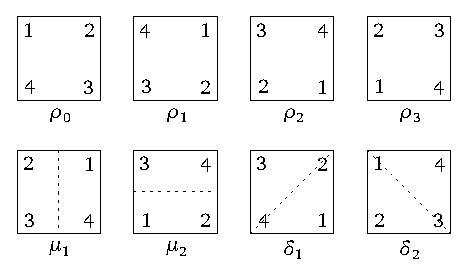
\includegraphics{wssquares.eps}
    \end{center}

\end{enumerate}
Redo the worksheet, and add cycle notation.

\chapter{Introduction to Groups}

\begin{definition}
    A \textbf{binary operation} \(*\) on a set \(A\) is a function \(A \times A \rightarrow A\), where \((a,b) \mapsto a*b\).  In other words, a binary operation inputs two elements \(a\), \(b\) of the set \(A\), and outputs a well-defined element \(a * b\) of the set \(A\).
\end{definition}

\begin{problem}\label{prob:binops}
Which of the following are binary operations on the specified set? If not, explain why not.
\begin{enumerate}
  \item Addition on \(\mathbb{Z}\), the set of integers.
  \item Subtraction on \(\mathbb{Z}\), the set of integers.
  \item Subtraction on \(\mathbb{N}\), the set \(\{1,2,3,\ldots\}\) of natural numbers.
  \item Division on \(\mathbb{R}\), the set of real numbers.
  \item Division on \(\mathbb{Z}\setminus \{0\}\).
  \item Composition on \(D_4\), the symmetries of the square.
  \item Composition on the set of rotations in \(D_4\).
  \item Multiplication modulo 6 on \(\mathbb{Z}_6\).
\end{enumerate}
\end{problem}

\begin{definition}
A binary operation is \textbf{associative} if \((a * b)*c = a*(b*c)\) for all \(a,b,c \in A\). An operation is \textbf{commutative} if \(a * b = b * a\) for all \(a,b \in A\). An element \(e\) is said to be an \textbf{identity} for~\(*\) if \(a*e = e*a = a\) for all \(a \in A\).
An element \(b\) is an \textbf{inverse} of the element \(a\) if \(a * b = b * a = e\).
\end{definition}

\begin{problem}
Refer back to those operations in Problem~\ref{prob:binops} that were binary operations.
Do the following for each of these binary operations.
\begin{enumerate}
  \item Determine whether the operation is associative, and if not, prove that the operation is not associative.
  \item State whether there is an identity for the operation, and if so, identify it.
  \item If there is an identity for the operation, determine which elements (if any) have inverses.
\end{enumerate}
\end{problem}

\begin{problem}
Determine which of the binary operations in Problem~\ref{prob:binops} are commutative, and if not, provide proof that the operation is not commutative.
\end{problem}

\begin{problem}
Prove that if a binary operation \(*\) on a set \(A\) has an identity element, then that identity element is unique.
\end{problem}

\begin{definition}
A \textbf{group} is a set \(G\) together with a binary operation \(*\) on \(G\) satisfying the following:
\begin{enumerate}
  \item The operation \(*\) is associative.
  \item There is an element in \(G\) which is an identity for \(*\).
  \item Every element in \(G\) has an inverse with respect to \(*\) in \(G\).
\end{enumerate}
We denote the group by \(\langle G, * \rangle\). We refer to the set \(G\) as the \textbf{underlying set} of the group \(\langle G, * \rangle\). (However if the specific operation is clear from the context, or is not important in the context, we sometimes simply write \(G\) instead of \(\langle G, * \rangle\) for the group, and speak of ``the group \(G\).'')
\end{definition}

\begin{problem}\label{prob:groupex}
Which of the following are groups? If not, explain why not.
\begin{enumerate}
  \item  \(\langle \mathbb{Z}, + \rangle\)
  \item  \(\langle \mathbb{Z}, - \rangle\)
  \item  \(\langle \mathbb{Z}, \times \rangle\)
  \item  \(\langle \mathbb{Z}, \div \rangle\)
  \item  \(\langle \mathbb{R}^+, \times \rangle\) (\(\mathbb{R}^+\) denotes the set of positive real numbers.)
  \item  The set of symmetries of a regular pentagon with operation composition.
  \item  \(\mathbb{Z}_6\) with operation addition mod 6.
  \item  \(\mathbb{Z}_6\) with operation multiplication mod 6.
  \item  \(\mathbb{Z}_6 \setminus \{0\}\) with operation multiplication mod 6.
  \item  \(\mathbb{Z}_5 \setminus \{0\}\) with operation multiplication mod 5.
\end{enumerate}
\end{problem}

\begin{problem}
Prove that the following is, or is not a group, as appropriate.
The set \( S = \mathbb{R} \setminus \{1\} \) with operation defined by \( a * b = a + b - ab \) for all \(a\) and \(b\) in \(S\). (On the right side of the equation, the operations are the usual addition and multiplication in \(\mathbb{R} \).)
\end{problem}

\begin{problem}
Prove that the following is, or is not a group, as appropriate: The set \(M_2(\mathbb{R})\) of all 2 by 2 matrices, with real numbers as entries, and operation matrix multiplication.
\end{problem}

\begin{definition}
\begin{itemize}
  \item A group \( \langle G, * \rangle \) is said to be \textbf{abelian} if \(*\) is commutative.
  \item We say a group is \textbf{finite} if the underlying set contains finitely many elements. We say a group is \textbf{infinite} if the underlying set contains infinitely many elements.
  \item For a finite group \(G\), the \textbf{order} of \(G\) is the number of elements in \(G\).
\end{itemize}
\end{definition}

\begin{problem}
Provide at least two examples of abelian groups.
\end{problem}

\begin{problem}
Refer back to question~\ref{prob:groupex}. Identify the finite groups in that question, and for each of these state the order of the group.
\end{problem}

\begin{problem}
Provide at least two examples of non-abelian groups. For one of these, prove that the group is non-abelian.
\end{problem}

\begin{problem}
Suppose \( \langle G, * \rangle \) is a group, with \(s\), \(t\) and \(u\) in \(G\). Prove or disprove as appropriate: If \( s * t = u * s \), then \(t = u\).
\end{problem}

\textbf{Remark: Using equations.} Let \(a, b, c\) be elements of a group \(G\). Since the binary operation in a group is well defined, it is OK to multiply both sides of an equation by the same element. In other words, \(a = b\) implies that \( c * a = c * b\) and \(a * c = b * c\).

\begin{problem}
Let \(G\) be a group, and let \(a \in G\). Prove that \(a\) has a unique inverse.
\end{problem}

\begin{problem}
Suppose \(G\) is a group, with \(a\) and \(b\) in \(G\). Prove that if \(a * b = e\), then \(b * a = e\). Use this to prove that if \(G\) is a group, with \(a\) and \(b\) in \(G\) and \(ab = e\), then \(a\) is the inverse of \(b\).
\end{problem}

\textbf{Notation:} For convenience, instead of using ``\(*\)'' to denote the group operation, we often use multiplicative notation as follows:
\begin{itemize}
  \item In place of \(a * b\) write \(ab\).
  \item Denote the inverse of \(a\) (the existence and uniqueness of which is ensured by Problem 12), by \(a^{-1}\).
  \item Let \(a^1\) denote \(a\), and for \(n \in \mathbb{N}\), with \(n > 1\), define \(a^n\) to be \(aa^{n-1}\).
\end{itemize}

It is important to note that we have simply introduced some notation; the operation ``multiplication'' in a group is NOT in general familiar old multiplication. Take care when working in an arbitrary group not to take for granted properties of exponents that are familiar from working with the real numbers. So for example, in the next two problems you may not assume that \(a^ma^n = a^{m+n}\), nor that \((a^m)^n = a^{mn}\).

\begin{problem}\label{prob:powinv}
In a group \(G\), if \(a \in G\) and \(n \in \mathbb{N}\), then both \( (a^n)^{-1}\) and \((a^{-1})^n\) have unambiguous interpretations in terms of the definitions above. Prove that these two are in fact equal.
\end{problem}

\begin{problem}
Prove that if \(G\) is a group, with \(a \in G\), then \((a^{-1})^{-1} = a\).
\end{problem}

You have shown in Problem~\ref{prob:powinv} that \((a^n)^{-1}\) and \((a^{-1})^n\) have unambiguous meanings, and are in fact equal. The symbol \(a^{-n}\), on the other hand, is not automatically defined by the definitions already given. It is convenient to define \(a^{-n}\) as simply another notation for \((a^n)^{-1}\) and \((a^{-1})^n\):

\textbf{Definition:} In a group \(G\) with \(a \in G\), we define \(a^{-n}\) to be \((a^n)^{-1}\). Also we define \(a^0\) to be the identity, \(e\).

As we've said, we cannot simply assume that exponents will have the same properties in an arbitrary group as they do when working with real numbers. Some familiar properties of exponents for real numbers are in fact false in certain groups. The next problem establishes two basic principles that \emph{do} apply in an arbitrary group.

\begin{problem}
Suppose \(G\) is a group, with \(a \in G\). Using notation like \[a^n = \underbrace{a * a * \cdots * a}_n, \] give a brief informal argument  that \(a^ma^n = a^{m+n}\) and \((a^m)^n = a^{mn}\) for all integers \(m\) and \(n\). (A formal proof requires a tedious but straightforward use of induction.)
\end{problem}

\begin{problem}
Suppose \(G\) is a group, with \(a\), \(b\), and \(x\) in \(G\). If \(x=a^{-1}b\), can we conclude that \(xa = b\)? Either prove this conclusion true, or provide a counterexample.
\end{problem}

\begin{problem}
Prove or disprove, as appropriate: Suppose \(G\) is a group, with \(a\), \(b\) and \(c\) in \(G\). If \(ac = bc\), then \(a = b\).
\end{problem}

\begin{problem}
Prove or disprove, as appropriate: If \(G\) is a group, with a and \(b\) in \(G\), then \((ab)^2 = a^2b^2\).
\end{problem}

\begin{problem}
Prove or disprove, as appropriate: If \(G\) is a group, with \(a\) and \(b\) in \(G\), then \((ab)^{-1} = a^{-1}b^{-1}\).
\end{problem}

\begin{problem}
Prove or disprove, as appropriate: If \(G\) is a group, with \(a\) and \(b\) in \(G\), then \((ab)^{-1} = b^{-1}a^{-1}\).
\end{problem}

Historically, the central focus of abstract algebra was the solution of equations. The following problem gives an indication of the connection:

\begin{problem}
Suppose \(G\) is group, with \(a\) and \(b\) in \(G\). Consider the equation \(ax = b\).
\begin{enumerate}
  \item Prove that \(a^{-1}b \in G\).
  \item Prove by substituting that \(x = a^{-1}b\) is a solution for the equation.
  \item Prove that \(x = a^{-1}b\) is the \emph{only} solution for the equation \(ax = b\); that is, this solution is \emph{unique.}
\end{enumerate}
\end{problem}

You have thus shown that if \(G\) is a group, then for all \(a\) and \(b\) in \(G\), there is a unique solution in \(G\) for the equation \(ax = b\). Similarly there is a unique solution in \(G\) for \(xa = b\).

\chapter{Mandatory Reading}

\section{Getting Started}

The base requirement is  a \LaTeX{} distribution. Once you have this, place the following
three files from \emph{www.jiblm.org/jiblm/info/authorinfo.aspx} into your working directory.

\begin{enumerate}
 \item \texttt{JIBLM.tex} -- This is the file containing additional \LaTeX{} commands
       beyond those of the standard book class in order to typeset a JIBLM document.  You should not need
       to edit this file.
 \item \texttt{template.tex} -- This file contains the text you are currently reading.
 \item A copy of \texttt{template.tex}, named \texttt{myfile.tex} or whatever you like.
\end{enumerate}

\noindent
You are now ready to edit \texttt{myfile.tex} which will become your submission.

\begin{enumerate}

 \item At the top of \texttt{myfile.tex}, locate
       \begin{verbatim}
  %%% Begin {Title Page} %%%%%%%%%%%%%%%%%%%%%%%%%%%%%%%%%
  \title{Author's Package}
  \author{Paul J. Kapitza}
  \affiliation{Berry College}
  \maketitle
  %%% End {Title Page} %%%%%%%%%%%%%%%%%%%%%%%%%%%%%%%%%%%
 \end{verbatim}
 and replace ``Author's Package", ``Paul J. Kapitza" and ``Berry
 College" with the title of your course notes, your name and your
 affiliation.

 \item Delete any of the subsequent content of \texttt{myfile.tex} that you wish with
       the exception of the commands \verb|\frontmatter|,
       \verb|\mainmatter|, \verb|\backmatter| and
       \verb|\end{document}| commands. The blocks of statements
       to be removed are easily identified as follows:
       \begin{center}
        \verb|%%%%%%%%%%%%%%%%%%%%%%BEGIN REMOVAL {n} %%%%%%%%%%%%%%%%%%%%%%|
        ....material to be removed....
        \verb|%%%%%%%%%%%%%%%%%%%%%END REMOVAL {n} %%%%%%%%%%%%%%%%%%%%%%%%%|
       \end{center}

\end{enumerate}

Your \texttt{myfile.tex} may now be filled in with your own course notes.

\section{Student and Instructor Versions}\label{ch:annotation}

You may wish to communicate with two different audiences, the students who
will study the materials and the instructors who will teach from the materials.
The \verb|\annotation| environment enables you to create one document that serves
as both a student and an instructor version.  By toggling a single comment in the preamble,
text and mathematics which is encased within the environment will be removed or restored
upon compilation, providing two versions from the same document.  Usage guidelines follow.

\begin{enumerate}


 \item To change versions, toggle the comment symbol between the following two lines in \texttt{myfile.tex}.

       \begin{center}
        \verb|%\StudentVersion|\\
        \verb|\InstructorVersion|\\
       \end{center}

 \item Use the \verb|\annotation| environment by placing opening and closing commands on lines
       separate from the material to be annotated, with no starting spaces or characters of any type
       on the lines containing the commands.  For example:

       \begin{center}
        \verb|\begin{annotation}|\\
        \verb|... your instructor-specific text goes here ...|\\
        \verb|\end{annotation}| \\
       \end{center}


 \item If a large comment is required, place the text in a separate file and use the commands:

       \begin{center}
        \verb|\begin{annotation}|\\
        \verb|\input{filename.tex}|\\
        \verb|\end{annotation}|\\
       \end{center}

 \item Numbered sequences should be handled with caution
       since the automatic numbering of Chapters, Theorems, Equations, etc., is recalculated when
       material is removed by the environment.

 \item While you may bracket anything you like using the \verb|\annotation{}| environment,
       such as comments within the theorem sequence, you may wish to add annotations
       to the instructor as footnotes throughout the text which can be made to appear as a chapter-like
       component at the end of the document.
\begin{annotation}
        \endnote{This is an example of a footnote to the instructor which will appear at the very
        end of the document.}
\end{annotation}
       This document has such a
       component entitled \emph{Notes to the Instructor} which will appear in the
       Instructor Version but not in the Student Version.
\begin{annotation}
        \endnote{This is another example of a footnote to the instructor, in case you missed the first one.}
\end{annotation}
       To do this:
       \begin{enumerate}
        \item  Insert in the text itself footnotes to the instructor
              in the following format.
\begin{verbatim}
\begin{annotation}
\endnote{This is an example of a footnote to the instructor.}
\end{annotation}
\end{verbatim}
        \item After the command \verb|\backmatter|, add the chapter-like component
              \emph{Notes to the Instructor} that you see following the
              \verb|\backmatter| command in \texttt{template.tex}.  Only do this if you have at
              least one endnote; otherwise you will get an error.
       \end{enumerate}
\end{enumerate}



\chapter{Optional Reading}

\section{Theorem-like Environments}

Theorem environments for declarations are provided and are numbered globally.
As an example of the \verb|\theorem{}| environment consider the following typesetting example.
\begin{theorem}
 (The Currant minimax principle.) Let $T$ be completely continuous self adjoint operator
 in a Hilbert space $H$. Let $n$ be an arbitrary integer and let $u_1,\ldots,u_{n-1}$ be
 an arbitrary system of $n-1$ linearly independent elements of $H$. Denote
 \begin{equation}
  \max_{\substack{v\in H, v\neq
   0\\(v,u_1)=0,\ldots,(v,u_n)=0}}\frac{(Tv,v)}{(v,v)}=m(u_1,\ldots, u_{n-1})
  \label{thm:minmax1}
 \end{equation}
 Then the $n$-th eigenvalue of $T$ is equal to the minimum of these maxima, when
 minimizing over all linearly independent systems $u_1,\ldots u_{n-1}$ in $H$,
 \begin{equation}
  \mu_n = \min_{\substack{u_1,\ldots, u_{n-1}\in H}} m(u_1,\ldots, u_{n-1}) \label{thm:minmax2}
 \end{equation}
\end{theorem}
Note: The above equations are automatically numbered as equation (\ref{thm:minmax1}) and
(\ref{thm:minmax2}).



A number of theorem-like environments are included for structuring mathematical statements.  Examples of these are given below in alphabetical order.

\begin{axiom}
 This is an axiom
\end{axiom}


\begin{definition}
 This is a definition
\end{definition}


\begin{lemma}
 This is a lemma
\end{lemma}

\begin{problem}
This is a problem
\end{problem}



\begin{theorem}[Main Theorem]
 This is a theorem
\end{theorem}

Additionally, {\bf acknowledgment}, {\bf algorithm}, {\bf case}, {\bf claim}, {\bf conclusion}, {\bf condition},
{\bf conjecture}, {\bf corollary}, {\bf criterion}, {\bf example}, {\bf exercise}, {\bf notation},
{\bf proposition}, {\bf remark}, {\bf solution}, {\bf summary}, and {\bf proof} are available.

\section{Packages, Commands, Styles, and Libraries}

\begin{enumerate}

 \item The following packages are used by the Journal:
       \begin{itemize}
        \item \texttt{book}--The base book class of \LaTeX.
        \item \texttt{time}--Make system time available.
        \item \texttt{enumerate}--Extended enumeration package.
        \item \texttt{amssymb}, \texttt{amsmath}, \texttt{latexsym}, \texttt{amsthm}--Symbol libraries.
        \item \texttt{lettrine}--Drop-caps.
        \item \texttt{mathptmx}--Times Roman type package for both math and text.
        \item \texttt{fancyhdr}--Header customization.
        \item \texttt{comment}--Base package for the annotation environment.
        \item \texttt{endnotes}--End notes package.
       \end{itemize}


 \item The current Journal Style does not contain any packages which support graphics content.
       To include this facility, place a \verb|\usepackage{pkg-choice}| command  directly after
       the first command line in your text file, \verb|\include{JIBLM}|.  Popular packages available
       include \texttt{graphics}, \texttt{graphicx} and \texttt{epsfig}.


 \item The following sectioning commands are available:
       \begin{itemize}
        \item \verb"\chapter{Chapter Title}" command produces a new chapter starting on a new page,
        \item \verb"\section{Section Title}" command for major sections, and
        \item \verb"\subsection{Subsection Title}" command for subsections.
       \end{itemize}

 \item Generally, all the styles available from \LaTeX{} are available, including:
       \begin{itemize}
        \item Typeset text shapes include \emph{Emphasize}, \textbf{Bold},
              \textit{Italics} and \textsl{Slanted} texts.
        \item You can also typeset \textrm{Roman}, \textsf{Sans Serif}, \textsc{Small Caps}, and
              \texttt{Typewriter} families.
        \item The size tags are available;  {\tiny Tiny},
              {\scriptsize Scriptsize}, {\footnotesize Footnotesize}, {\small Small}, {\normalsize
               Normalsize}, {\large Large 1}, {\Large Large 2 }, {\LARGE Large 3}, \ {\huge Huge 1} and {\Huge
              Huge 2}.

       \end{itemize}

 \item The symbol libraries included within the journal package are the
       \texttt{amssymb}, \texttt{amsmath}, \texttt{latexsym} and \texttt{amsthm} packages.
       This collection provides for most of the commonly used mathematical typesetting tools to be
       directly accessed. Consult your favorite \TeX{} reference for details.   Of particular interest
       are the mathematical styles,
       \begin{enumerate}
        \item $\mathbb{BLACKBOARD}$, (e.g., $\mathbb{R}\,$,$\mathbb{Z}\,$,$\mathbb{C}$).
        \item $\mathcal{CALLIGRAPHIC}$, (e.g. $\mathcal{S}= \emptyset$), and
        \item $\mathfrak{Fraktur}$.
       \end{enumerate}



\end{enumerate}
%%%%%%%%%%%%%%%%%%%%%%%%%%%END REMOVAL {4} %%%%%%%%%%%%%%%%%%%%%%%%%%%%%%%%%


%%%%%%%%%%%%%%%%%%%%%%%%%%%BEGIN REMOVAL {5} %%%%%%%%%%%%%%%%%%%%%%%%%%%%%%%%%
\backmatter

\begin{annotation}
 \chapter{Notes to the Instructor}

 \renewcommand\notesname{}
 \vspace{-2cm}
 \begingroup
 %\setlength{\parindent}{0pt}% Don't know what this does.  DMC
 \setlength{\parskip}{2ex}
 \renewcommand{\enotesize}{\normalsize}
 \theendnotes
 \endgroup
\end{annotation}

\vspace{.1in}

You can also add any text you want here.

%%%%%%%%%%%%%%%%%%%%%%%%%%%END REMOVAL {5} %%%%%%%%%%%%%%%%%%%%%%%%%%%%%%%%%

\end{document}
